\documentclass[12pt]{report}

\usepackage[utf8]{inputenc}



\usepackage[a4paper,  total={6in, 8in}]{geometry}



\usepackage{ragged2e} %--For text alignment

\newenvironment{frontmatter}{}{\maketitle}

\usepackage{longtable}

\usepackage{graphicx}
\usepackage{rotating}
\usepackage{amssymb,amsmath}
%% The lineno packages adds line numbers. Start line numbering with
%% \begin{linenumbers}, end it with \end{linenumbers}. Or switch it on
%% for the whole article with \linenumbers after \end{frontmatter}.
%\usepackage{lineno}
\newtheorem{theorem}{Definition}
\usepackage{subfigure}
\usepackage{lscape}
%\usepackage{datetime}

%\usepackage{fancyhdr}
% 
%\pagestyle{fancy}
%\fancyhf{}
%\rhead{Put your tit}
%\lhead{Title}
%\rfoot{Page \thepage}


\begin{document}

\begin{titlepage}
\begin{center}
%\vspace*{0.5cm}

\textbf{ {\fontsize{18pt}{12pt}\selectfont TITLE OF PROJECT REPORT}}
        
\vspace{0.5cm}
        
\textbf{ {\fontsize{14pt}{12pt}\selectfont A PROJECT REPORT}}

\vspace{1.5cm}

 {\fontsize{14pt}{12pt}\selectfont Submitted by}\\
 \vspace{0.5cm}
 {\fontsize{16pt}{12pt}\selectfont Name of the Candidate (s)
 }\\       
\vspace{1.5cm}

{\fontsize{14pt}{12pt}\selectfont Supervised by}\\
\vspace{0.5cm}
{\fontsize{14pt}{12pt}\selectfont Name of Faculty
}\\
\vspace{0.5cm}
{\fontsize{14pt}{12pt}\selectfont in partial fulfillment for the award of the degree}\\
\vspace{0.5cm}
{\fontsize{14pt}{12pt}\selectfont of}\\
\vspace{0.5cm}
{\fontsize{14pt}{12pt}\selectfont NAME OF THE DEGREE 
}\\
\vspace{0.5cm}
{\fontsize{14pt}{12pt}\selectfont IN}\\
\vspace{0.5cm}
{\fontsize{14pt}{12pt}\selectfont Branch of Study}\\
\vspace{0.5cm}
{\fontsize{14pt}{12pt}\selectfont Year: 2024}\\
%\vspace{0.5cm}

\vfill
       
\vspace{0.3cm}
        

\includegraphics[width=0.25\textwidth]{Makaut_logo.jpg}
        
Dept of Computer Applications\\
School of Information Science and Technology\\
Maulana Abul Kalam Azad Univerity of Technology\\
Nadia, West Bengal, India\\
    
       {MAY}{\hspace*{0.5cm}}{2015}
       %\date{\displaydate{date}}
        
    \end{center}
\end{titlepage}
\newpage

\pagenumbering{gobble} 

\begin{center}
\vspace*{8.5cm}
\LARGE
\textit{Dedicated to my Parents}

\end{center}

\newpage


 \begin{center}
        \vspace*{1cm}
         \LARGE
        \textbf{BONAFIDE CERTIFICATE}
        
        \vspace{1.5cm}
 \justify    
 {\fontsize{14pt}{12pt}\selectfont 	
 Certified that this project report ``TITLE OF THE PROJECT" is the bonafide work of ``NAME OF THE CANDIDATE(S)" who carried out the project work under my supervision.}\\  
	        
        
        \vspace{2.5cm}
 \normalsize    
 \begin{minipage}{3in}
 	\textbf{\underline{Signature of the HoD}} \\
 	Dr. Sayani Mondal\\
 	Assistant Professor, Dept of ET,\\ 
 	HoD, Dept of Computer Applications,\\
 	Maulana Abul Kalam Azad University of Technology
 \end{minipage}
 \hfill
 \begin{minipage}{2.5in}
 	\textbf{\underline{Signature of the Supervisor}} \\
 	Dr. Pabitra Pal\\
 	SUPERVISOR\\
 	Assistant Professor,\\
 	Dept of Computer Applications,\\
 	 	Maulana Abul Kalam Azad University of Technology
 \end{minipage}
        
     \vspace{2.5cm}    
  \begin{minipage}{3in}
  	\textbf{\underline{Signature of External Examiner}} \\
  	
  \end{minipage}     
        
        
    \end{center}

\newpage


\begin{center}
        \vspace*{1cm}
         \LARGE
        \textbf{Declaration}
        
        \vspace{1.5cm}
 \justify 
 {\fontsize{14pt}{12pt}\selectfont I hereby declare that this submission is my own work and that, to the best of my knowledge and belief, it contains no material previously published or written by another person nor material which has been accepted for the award of any other degrees or diplomas of the university or other institutes of higher learning, except which due acknowledgment has been made in this text.         
 }\\     
		
        \vspace{5.5cm}
      
      
   \begin{minipage}{3in}
 	\textbf{\underline{Signature of the Candidate}} \\

 	   Name of the Candidate
 \end{minipage} 
        
        \vfill
        
       
        
        
        
    \end{center}

\newpage

\begin{center}
        \vspace*{1cm}
         \LARGE
        \textbf{Acknowledgments}
        
        \vspace{1.5cm}
 \justify   
 {\fontsize{14pt}{20pt}\selectfont I hereby wish to express my sincere gratitude and respect to Assistant \textbf{NAME of SUPERVISOR}, Dept. of Computer Applications, SIS\&T, MAKAUT under whom I had proud privilege to work. His valuable guidance and encouragement have really led me to the path of completion of this project. Any amount of thanks would not be enough for the valuable guidance of my supervisor. \\
 I would also like to thank all the faculty member of CA dept. for their devoted help. I also cordially thank all laboratory assistants for their cooperation.\\
 Finally, I would like to pen down my gratitude towards my family members for their continuous support and encouragement. It would have not been possible to complete my work without their support. }     
		
   
        
     
        
       \vfill
        
       
        
        
        
    \end{center}
    


\newpage
\vspace*{1cm}
\begin{center}
\LARGE
\textbf{Abstract}
\end{center}

\justify
 your abstract begins here.........\\
 Write your abstract in maximum 200-300 words.
 
 \vspace*{1cm}
 \smallskip
\noindent \textbf{Keywords.} list of keywords.
 Put atleast 6-8 keywords of your thesis work separated by coma(,)
 

\newpage
%\addcontentsline{toc}{chapter}{*}
\tableofcontents



\listoffigures


\newpage

\listoftables

\newpage
%\setcounter{page}{1}
\pagenumbering{arabic}
\chapter{Introduction}
%\justify
\section{ARRANGEMENT OF CONTENTS:}

The sequence in which the project report material should be arranged and bound should be as follows:


\begin{itemize}
	\item Title Page
\item Bonafide Certificate
\item Acknowledgement (with names of students at the bottom)
\item Table of Contents
\item List of Tables
\item List of Figures
\item List of Symbols, Abbreviations and Nomenclature
\item Abstract
\item Chapters
\item Appendices
\item References
\end{itemize}

The table and figures shall be introduced in the appropriate places.
\section{PAGE DIMENSION AND BINDING SPECIFICATIONS:}


The dimension of the project report should be in A4 size.   The project report should be spirally bound. The cover should be printed in black letters and the text for printing should be identical. 


\newpage

\chapter{Background Theory}

{\bf Mathematical Equations}\\

You can write your mathematical equation as like in Eq.(\ref{eq:1}).

\begin{equation}
\label{eq:1}
X_{i}^{2}+Y_{j}^{2}=Z_{k}^{2}
\end{equation}


\newpage

\chapter{Review}

\newpage
\chapter{Materials \& Methods}
\section{Example of Table}



\begin{table}[h]
\centering
\caption{Table to test captions and labels}
\label{table:1}
\begin{tabular}{ |c| c| c| }
\hline
 cell1 & cell2 & cell3 \\ 
 \hline
 cell4 & cell5 & cell6 \\ 
 \hline 
 cell7 & cell8 & cell9   \\ 
 \hline
\end{tabular}

\end{table}




The table \ref{table:2} is an example of referenced \LaTeX elements.
\begin{sidewaystable}[h]
%\begin{table}[]
\centering
\caption{Table to test captions and labels}
\label{table:2}
\begin{tabular}{ |c| c| c| }
\hline
 cell1 & cell2 & cell3 \\ 
 \hline
 cell4 & cell5 & cell6 \\ 
 \hline 
 cell7 & cell8 & cell9   \\ 
 \hline
\end{tabular}

%\end{table}
\end{sidewaystable}




{\bf Multi-page tables}\\

If you have to insert a very long table, which takes up two or more pages in your document, use the longtable package. First, add to the preamble the line

\begin{verbatim}
\usepackage{longtable}
\end{verbatim}


\begin{longtable}[c]{| c | c |}
 \caption{Long table caption.\label{long}}\\
 
 \hline
 \multicolumn{2}{| c |}{Begin of Table}\\
 \hline
 Something & something else\\
 \hline
 \endfirsthead
 
 \hline
 \multicolumn{2}{|c|}{Continuation of Table \ref{long}}\\
 \hline
 Something & something else\\
 \hline
 \endhead
 
 \hline
 \endfoot
 
 \hline
 \multicolumn{2}{| c |}{End of Table}\\
 \hline\hline
 \endlastfoot
 
 Lots of lines & like this\\
 Lots of lines & like this\\
 Lots of lines & like this\\
 Lots of lines & like this\\
 Lots of lines & like this\\
 Lots of lines & like this\\
 Lots of lines & like this\\
 Lots of lines & like this\\
 ...
 Lots of lines & like this\\
 \end{longtable}

%The table \ref{table:3} is an example of referenced \LaTeX elements in landscape.
%
%\begin{landscape}
%
%\begin{table}[bth]
%\begin{center}
%\caption{Table to test captions and labels}
%\label{table:3}
%\begin{tabular}{ |c| c| c| }
%\hline
% cell1 & cell2 & cell3 \\ 
% \hline
% cell4 & cell5 & cell6 \\ 
% \hline 
% cell7 & cell8 & cell9   \\ 
% \hline
%\end{tabular}
%
%\end{center}
%\end{table}
%
%\end{landscape}

\newpage

\chapter{Results \& Discussion}

The graph is given in Fig.~\ref{fig:logo}.

\begin{figure}[!bth]
\center
\label{fig:logo}
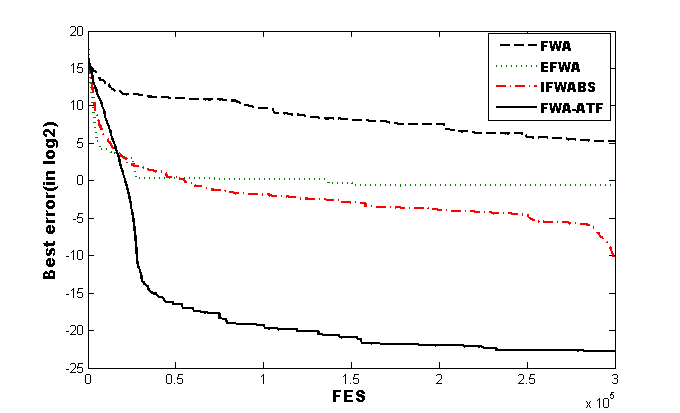
\includegraphics[scale=0.6]{f1.png}
\caption{Graph}
\end{figure}


If you need to place multiple images all together, use this...


\begin{figure}[!h]
  \centering
   \begin{tabular}{l l l}
  \subfigure[\label{db1mri1}]{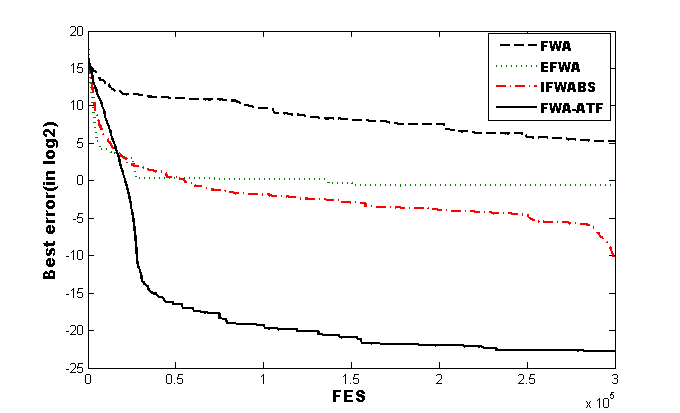
\includegraphics[width=1.4in,height=1.2in]{f1.png}}   &
   
  \subfigure[\label{db1mri2}]{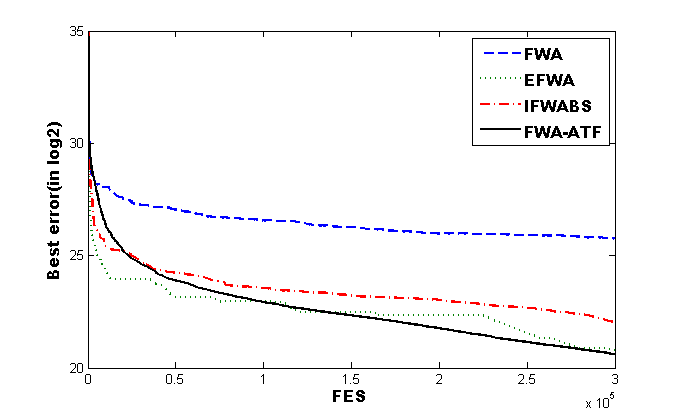
\includegraphics[width=1.4in,height=1.2in]{f2.png}}   &
 
  \subfigure[]{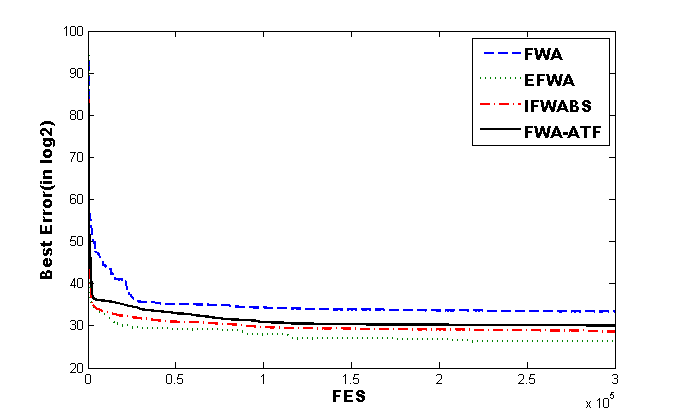
\includegraphics[width=1.4in,height=1.2in]{f3.png}}  \\

  \subfigure[]{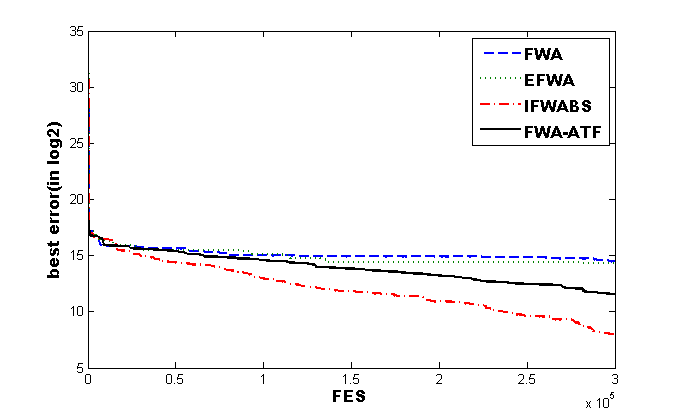
\includegraphics[width=1.4in,height=1.2in]{f4.png}}   &
 
  \subfigure[]{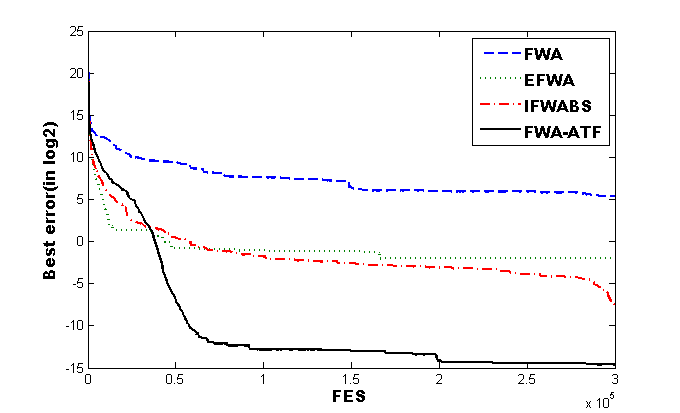
\includegraphics[width=1.4in,height=1.2in]{f5.png}}   &

  \subfigure[]{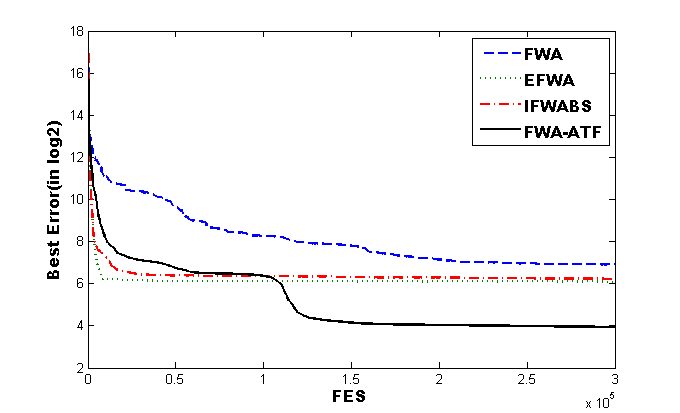
\includegraphics[width=1.4in,height=1.2in]{f6.png}}   \\
   \end{tabular}   
  \caption{put the caption}.
 \label{fig:db1}
\end{figure}



\newpage

\chapter{Conclusions}

\newpage

\chapter{Future Works}
Here you can outline the future scopes of your work..........
\newpage

\chapter*{List of Publications}
\begin{enumerate}
\item Author's name, Title, Conference, date, place, year, pp.~xx-xx.
\item Author's name, Title, Journal, Vol~X, No.~X, Year, pp.~xx-xx.
\end{enumerate}
\newpage
\bibliographystyle{plain}
%\begin{thebibliography}{plain}
\bibliography{Bibliography}


\end{document}
